This chapter discusses related work in the field of digital preservation. First some general information about projects and activities are presented and then an overview of the most common approaches of dealing with digital content in the long-term are outlined. Then a definition of the term collection is given and important aspects, such as meta data, its analysis and scalability are discussed. Following the chapter gives an overview of the current state of the art in tool support and discusses the influence and importance of quality assurance of measurements with respect to content profiling. At the end, the author gives some personal observations about the state of the art and the identified problems and gaps.

\section{Preservation}
More and more information is produced in digital form and more and more information has only a digital representation. This has enormous implications for national and state archives, libraries, scientific institutions and business enterprises but also the small companies and even private people as they often face data corruption and access problems in the long-term.
In general, digital preservation (or DP for short) copes with two main problems; preserving content (bit streams) for longer periods of time and ensuring these contents are accessible and understandable in the future. When talking about ``the future'' or ``longer periods of time'' we mean ``as long as the content is needed''.
Of course this view is over simplified and there are many more challenges in digital preservation. From the fundamental technical problems through organisational and social challenges to practical and financial ones.

A good example to picture the problem and challenges in DP is presented in \cite{Lorie:2001:LTP:379437.379726} and in \cite{Rauber:2009:dpchallenges}. Imagine a file created today on a specific physical machine. This file is nothing more than a series of bits shaped in a specific format. In order to access this file in the long term, not only the bits and bytes have to be preserved but also the way of interpreting them (the format specification). This would also require to preserve the programs that can open, render and manipulate the file, which in turn will require the preservation of the dependency libraries and software packages as well as the operating system and the whole environment in which these programs or program versions run. Failing to preserve only one single part of this chain and the file would be lost (even if the physical bit stream is still in tact).

Due to this and many other problems a community of preservation experts has emerged. Through the last decade a number of DP-related research projects and initiatives have been established. These have identified problems and threats and have advanced the state of the art in this filed. An overview of the EU DP projects and activities is presented in \cite{strodl:2011:dpreport}. Starting in the mid nineties scientists recognised that these problems could lead to disasters and thus the need of digital preservation and its importance. By the beginning of the new millennium there were the first initiatives and projects in the EU that started focusing on research topics related to DP aiming the establishment of a community, identification of target groups and transfer of expertise (ERPANET\footnote{http://www.erpanet.org/}, DELOS\footnote{http://www.delos.info/}, DPE\footnote{http://www.digitalpreservationeurope.eu/}). The first scientific research was focused on topics such as standards, system concepts, selection and appraisal policies and format identification. Afterwards more technical and practical approaches were undertaken to research the preservation of simple digital objects such as office documents and images (PLANETS\footnote{http://www.planets-project.eu}, CASPAR\footnote{http://www.casparpreserves.eu}). All this helped the establishment of a solid community and a body of expertise.

Present initiatives include more fundamental research that tries to focus rather on more complex and interactive objects than simple documents and data structures. Projects such as LiWA\footnote{http://www.liwa-pro ject.eu} attempt to solve issues related to Web Archiving whereas projects such as TIMBUS\footnote{http://timbusproject.net} and WF4Ever\footnote{http://www.wf4ever-pro ject.org} focus on the preservation of business processes and scientific workflows.
Other projects such as SCAPE\footnote{http://scape-project.eu} build upon the solid framework established in the past and aim to improve the state of the art of DP by developing infrastructure and tools for scalable preservation actions and integrating them with automated policy based preservation planning and preservation watch systems and workflows.
%what does the future hold

\subsection{Most Common Approaches}
% the tools at hand, why are these important, trade offs
Through the years many tools and procedures were developed in order to preserve digital content. In the literature there are often different names for the same concepts. Here we present the most prominent ones. \newline

\textit{Bit-Stream Preservation}
is the concept of copying the bits to a different medium with a different (physical) location. There are many different media which can store digital data. Some are more stable than others, some are more popular than others. No matter on what type of medium is chosen for data storage, CDs, DVDs, HardDrives, etc., it is not guaranteed that the data stream is safe. Through physical damage, bit rot or other disasters, there is a high chance that your digital storage media will fail to reproduce your bit stream. Thus on this lower level the only option would be to copy the streams to a different medium from time to time. This is strategy is often referred to as \textit{refreshing} \cite{Lee:2002:SOTADP}.

However, refreshing the data does not guarantee that it will be accessible in a later point in time as new media are also error prone. Therefore, approaches like LOCKSS (Lots Of Copies Keep Stuff Safe) \cite{reich2001lpw} make use of the distribution of many independent copies. Developed at the Stanford University the LOCKSS approach was implemented in a librarian software system that deploys many low cost copies of persistent web-caches and enables the detection and repair of damages based on voting in opinion polls \cite{Maniatis:2003:PPR:1165389.945451}.
%eventually say other projects that use LOCKSS (ExLibris, JISC, Hoppla, etc.)
Following a LOCKSS approach, however, only minimises the risk of losing data. If there is no effort spent in management of the copies, then it is fairly easy to lose track of the copies. For a software tool this might seem irrelevant but for a private user this is a real issue. Furthermore, even if enough well-managed copies have been stored and the data stream has been preserved, there is always the issue of software obsolescence and thus failure in the access and interpretation of the stream. \newline

\textit{Logical Preservation} tries to cope exactly with this problem. In order to preserve not only the bit stream, but also to ensure the integrity of a digital object and its successful interpretation in the long-term a migration approach is used \cite{Lee:2002:SOTADP}. New operating systems, new software tools or new versions are sometimes incompatible or unable to render and manipulate older formats. To cope with technology changes, digital preservation often uses a conversion strategy where the data is migrated (moved) to another format that is usually considered to be more stable than the original. A format is considered worthy and stable for preservation purposes when it is standardised, the format specification is open and well-documented, there are no patent owners and license fees that apply. The Florida Center for Library Automation, for example, offers a report\footnote{http://fclaweb.fcla.edu/uploads/recFormats.pdf} with the recommended data formats for preservation purposes that is considered as a good reference and starting point. However, there is no ultimate reference table or no ultimate file format that fits all preservation purposes. From use case to use case different aspects have to be considered. Neither standards, nor migration tools alone can ensure that a digital document remains accessible and its integrity remains unharmed. Wing and Ockerbloom further discuss the topic as they analyse what information is preserved by type converters and formalise the notion of respectful type converters in \cite{859529}. Informally a migration tool (or a converter) respects a certain type T if an original object A and a converted object B show the same behaviour when viewed as objects of type T. Rothenberg gives a good overview of common flaws of the concepts of logical preservation in \cite{rothenberg:1999:ensuring} and summarises important aspects that should be considered in DP. 

Nonetheless, logical preservation is often applied within digital preservation systems and repositories. As it also has potential pitfalls, it is not to be taken lightly.
Another more practical downside to migration are the storage costs. Often the target format has a bigger footprint than the original. Also the conversion of huge amounts of data is an error prone process that is not easy to validate \cite{Lorie:2001:LTP:379437.379726} and thus the originals are often kept for a certain period of time after the migration. Furthermore, if the migration path consists of several steps one has to make sure that all required meta data of the original is also migrated to the new versions of the objects. Another related issue is also quality assurance. As it is infeasible to check manually if the conversion process was successful, there are very specific requirements and processes that have to be followed in order to automate the verification of the preservation action \cite{feng:2010:qrofm}.
All these and other issues have to be carefully taken into account before choosing such a preservation action.
\newline

\textit{Emulation} has the verb ``emulate'' in its root, which means to imitate or reproduce.
In software terms, an emulator is a software tool that imitates the behaviour of a (hardware) system/framework (usually an older one) in order to run other (obsolete) tools that are meant to run on the emulated system. Clearly, this approach can come in handy in some DP activities.
In \cite{rothenberg:1999:ensuring} Rothenberg gives an overview of a process for preservation that is based on an emulation process. The author states that not only the data (bit-stream) has to be stored but also the bit stream of the original program, the operating system and all other necessary parts, e.g. dependencies and used libraries. Also a thorough and complete description and specification of the underlying architecture have to be provided in a form that is readable by potential future emulator authors. If these prerequisites are met, an emulator that mimics the specific hardware needed to run the tool can be created.
Lorie points out in \cite{Lorie:2001:LTP:379437.379726} that the specification of the architecture has to be perfect and complete, which is an immensely difficult task. Another very important argument he makes is the evaluation of such an emulator. Even if all needed input existed and a hypothetical emulator was created, how can its correctness be proven as no original hardware device exists?

These and other reasons combined form one of the biggest downsides of emulation; cost. The effort, manpower and infrastructure needed to emulate an environment that renders digital documents is often more expensive than the value of the content of the documents themselves.

Nevertheless, emulation is widely used in specific branches, such as video gaming.
Guttenbrunner et al have evaluated different strategies for the preservation of console video games in \cite{guttenbrunner:2008:evaluating} and came to the conclusion that while migration shows very good results for the preservation of visual and audio components it completely fails in interactivity. Emulation, on the other hand, showed promising results. All of these, however, were strongly dependent on the sample objects that were emulated.
%TODO stress more on the last statement

\subsection{Preservation Planning}
Preservation planning is a key task in DP that has to be undertaken by every institution or person that is serious about preservation. Numerous DP related projects have investigated the key requirements and processes involved in preservation planning. Projects such as PLANETS\footnote{http://www.planets-project.eu/} have created very strong fundaments in this area and have developed tools such as PLATO\footnote{http://ifs.tuwien.ac.at/dp/plato} - the preservation planning tool which supports a special workflow and helps users throughout numerous steps with the goal of creating a preservation plan. Follow up projects, such as SCAPE\footnote{http://www.scape-project.eu/} advance the state of the art and enhance the planning capabilities by improving the current status, by building up a framework around the process that supports many new features such as preservation monitoring services and by automating the whole process in order to provide a scalable, robust preservation planning process.\newline

\noindent\textit{What is Preservation Planning?}\newline
The OAIS reference model was developed by the Consultative Committee for Space Data Systems and soon afterwards was dubbed to be an ISO standard \cite{iso:2003:oais}. This high-level reference model has proven to be a helpful tool for the DP community for many years. Undoubtedly, one of its key parts is Preservation Planning or PP for short.

It is a decision making process that evaluates different preservation strategies or actions and chooses the most appropriate one. This process is highly dependent on object characteristics and institutional settings and requirements \cite{STR07_jcdl}. The goal of the process is to create a preservation plan that documents all the steps and choices that were made, the policies that were followed while making these decisions and the different preservation alternatives that were evaluated. It offers a complete documentation of the decision that allows one to repeat all experiments and verify why a certain preservation action was chosen.

The preservation plan is a very concrete artefact, opposed to policy documents, that specifies an action plan for the preservation of a set of digital objects.
\begin{quote}
A preservation plan defines a series of preservation actions to be taken by a responsible institution due to an identified risk for a given set of digital objects or records (called collection). The Preservation Plan takes into account the preservation policies, legal obligations, organisational and technical constraints, user requirements and preservation goals and describes the preservation context, the evaluated preservation strategies and the resulting decision for one strategy, including the reasoning for the decision. It also specifies a series of steps or actions (called preservation action plan) along with responsibilities and rules and conditions for execution on the collection. Provided that the actions and their deployment as well as the technical environment allow it, this action plan is an executable workflow definition \cite{Becker:2009fk}.
\end{quote}

%TODO describe more...
\begin{figure}[th]
\begin{center}
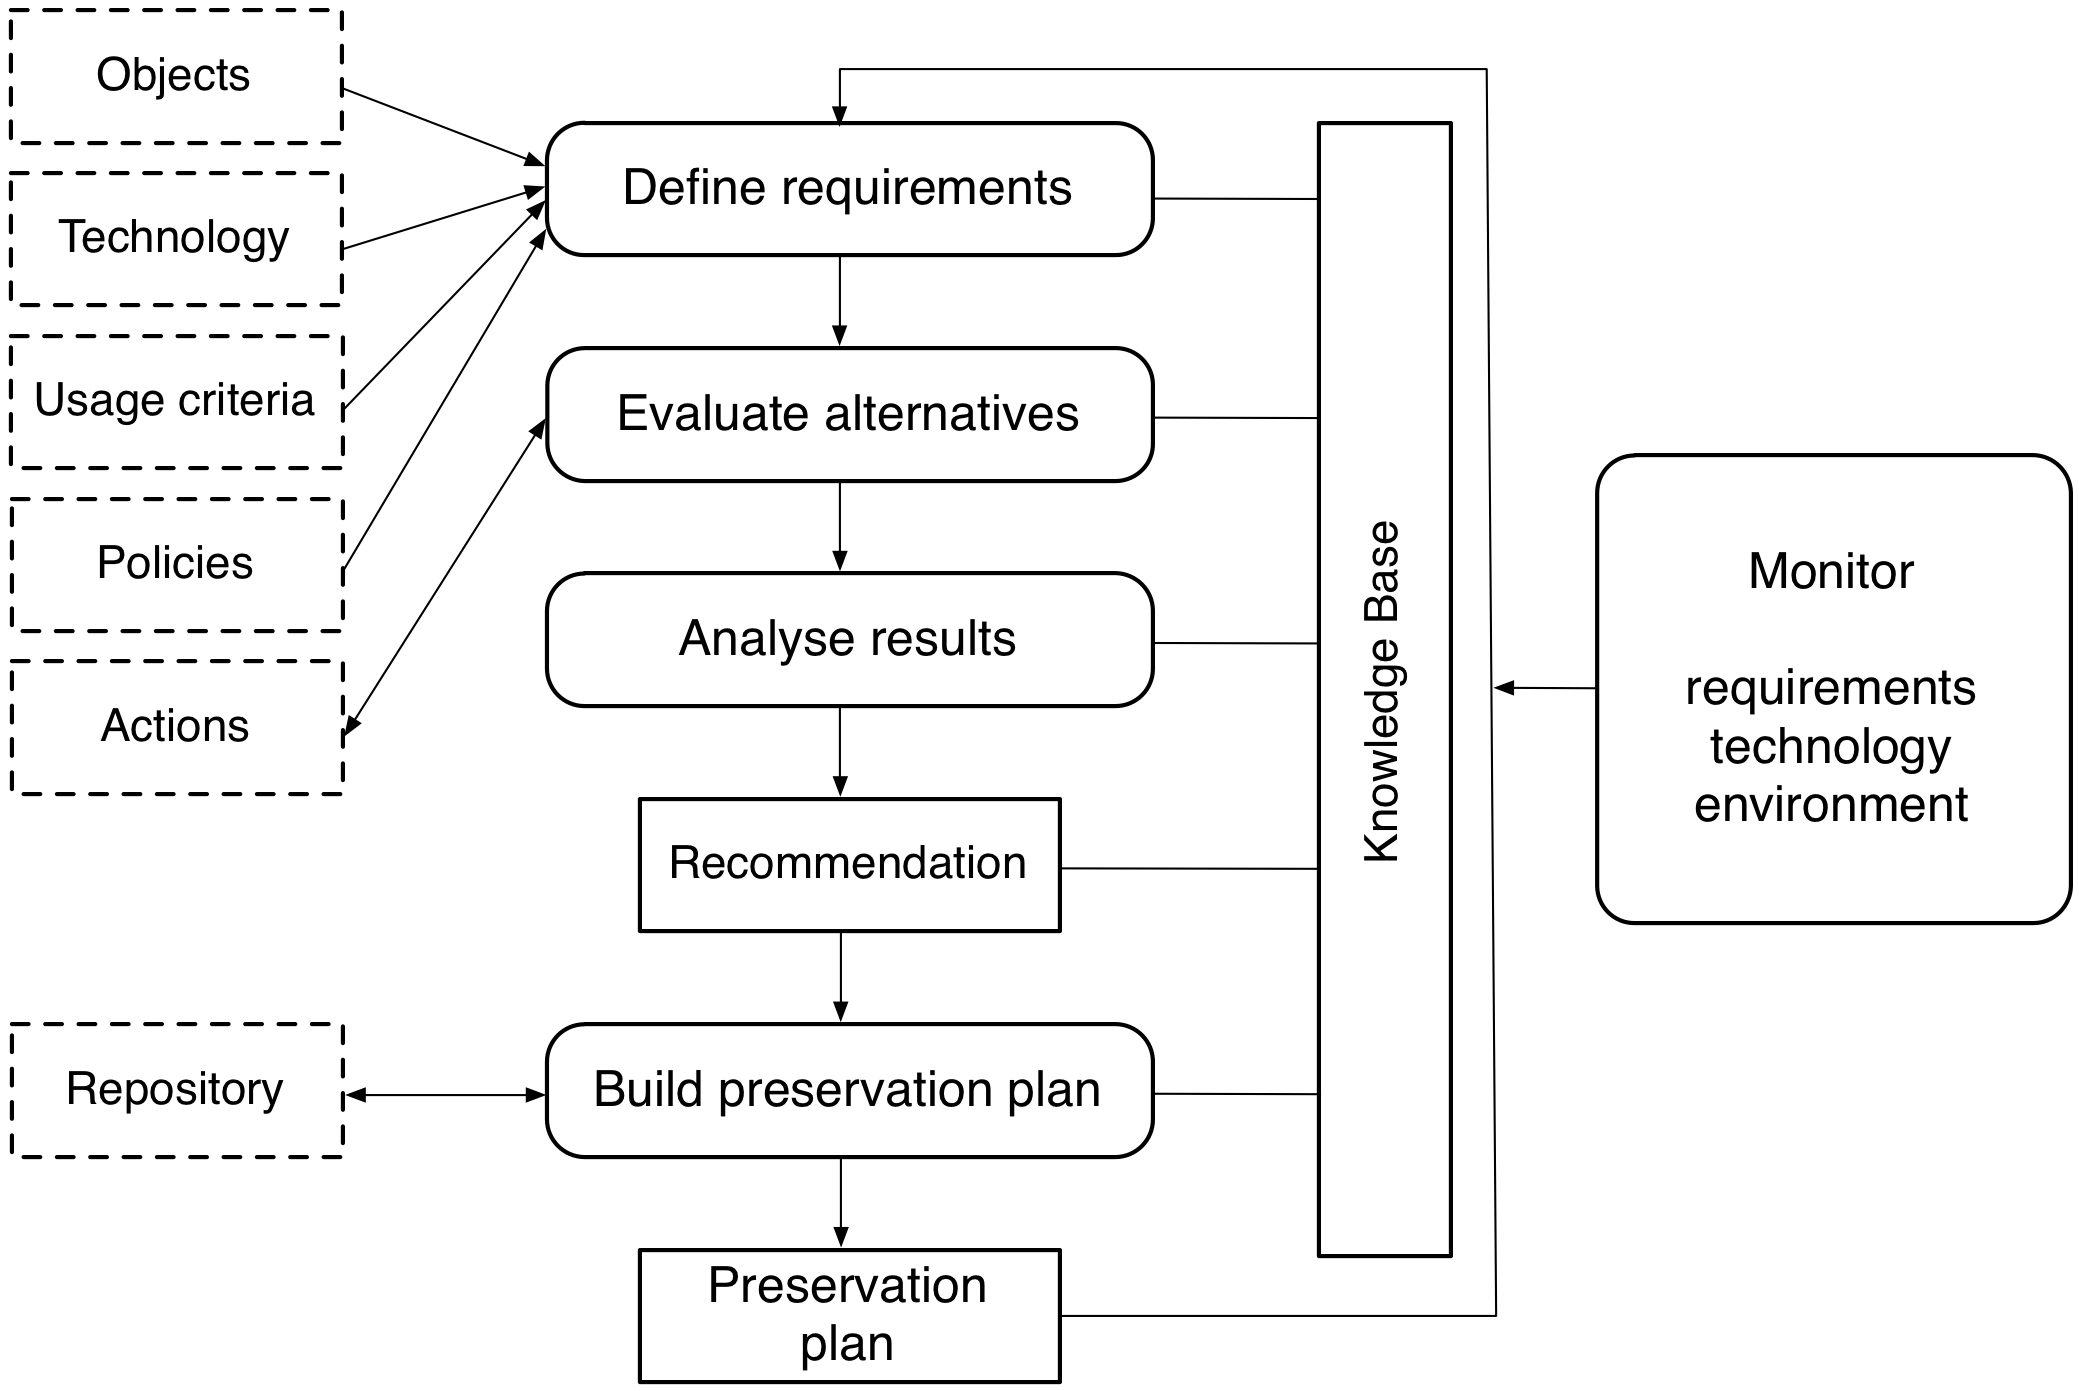
\includegraphics[width=4.0in]{figures/related/planningenvironment.png}
\caption{The preservation planning environment \cite{becker:2010:trustowrothy}.}
\label{fig:planenv}
\end{center}
\end{figure}

PLATO\footnote{http://ifs.tuwien.ac.at/dp/plato} is an online tool developed at the University of Technology in Vienna, which supports the whole preservation planning workflow.
It guides the user through all necessary steps to create a fully documented (and executable) preservation plan. The workflow follows a process specific to a preservation planning environment as the one in figure \ref{fig:planenv}. The process constitutes four main phases: define requirements, evaluate alternatives, analyse results and build preservation plan, all of which are covered by PLATO with respect to the context of the current use case, such as the objects, the current technology, policies, etc.
There is also an external monitoring phase which feeds back important information about relevant changes in the environment, which can cause a reiteration/reevaluation of a preservation plan. A detailed overview and a high level design of such an addition to the preservation planning environment can be found in \cite{duretec:2012:watch}.

%A key aspect of a preservation plan is the description of the collection. It includes general characteristics and allows the stratification of sample objects, which are the basis for the experiments and evaluation of the potential preservation actions.


%what it is, overview, steps, Plato, etc.
% the big picture
\section{Content}
%A collection here is defined as a set of digital objects that was created by some process or a user for some specific reason. Whether all digital objects are stored on the same physical location, how they are managed is irrelevant in this context. It is important to keep in mind that a set of digital objects exists and all of its objects are related for some reason.
In order, to create and analyze a collection or a set of digital objects the meta data for each object has to be examined. Meta data is a structured information about the data (objects) itself. It is usually stored within a file, that provides further information about the content and format of the file as well as other important characteristics. In general, there are three main types of meta data: descriptive meta data for discovery and identification (e.g. title, author, etc.), structural meta data (page ordering, image width and height, etc.), and administrative meta data that helps management of the resource (e.g. creation date, type, etc.). The National Information Standards Organisation - NISO\footnote{http://niso.org} has provided a series of articles and reports in order to help people, archivists and experts understand meta data and its importance \cite{citeulike:6387279}.

Today, analysis of such huge content often is done in a manual fashion, which can be a very time-consuming and cumbersome task. If there would be tools at hand that support identification and characterisation, data aggregation, filtering, collection splitting, etc., the the analysis process will be automated to a certain degree, hence analysis will be handled much faster and potentially much more efficient. 

It is noteworthy, that content here neither refers to the semantics of the information stored within the digital objects, nor to their visual representation characteristics or anything similar, but solely to the definition of the collection in terms of meta data, such as formats and format-related characteristics.

Consider a collection of digital scans of old newspapers. Its content here does not refer to the content of the newspapers, but to the meta data characteristics of the images that comprise the collection. For example, these may include, but are not necessarily restricted to the resolution of the scanned documents, their colour profiles, the scanning software, etc. All these measurements play a huge role in the decision making process of preservation planning.

The following paragraphs provide more details on metadata and how this refers to content profiling for preservation planning.

\subsection{Identification vs. Characterisation}
Based on different properties/characteristics a collection can be dubbed homogeneous or heterogeneous. Usually to a user a homogeneous collection would be a set of files that consists only or mostly of objects having the same format or even the same type (audio, video, text, etc.). This however, is an oversimplification, which has enormous side effects for preservation planning.

Consider the following example where a collection consists of N digital objects, which share the same extension, e.g. 'pdf'. To a normal user, this would be a homogeneous collection. An advanced user, however, would know that the extension of a file does not really specify the format of the file and thus could assume that there are differences.
One step further would be to conduct an identification process that looks for the specific file format and format version. Assume that in our example 95\% of all files have the same pdf format and format version.  Then this could be considered a homogeneous collection with respect to the format. 
In a next step, however, characterisation is conducted and now there are many more properties, such as \textit{creating applications}, \textit{encryption}, \textit{password protection}, \textit{tags}, etc.
Regarding these characteristics, the same collection can be considered to be heterogeneous.
Clearly, all of this is very important to preservation planning, since different preservation actions produce different results exactly because of such differences.

Thus the question remains, how to identify such important properties that define the homogenity of a collection? Following this train of thought, clearly the format is a very important characteristic. However, it does not cover all cases (as in the example) and many others are important.
% what is important here
% what is identification, what is characterization.
% meta data, distributions, aggregations, scalability, etc.
% homgeneous vs heterogeneous collections
% some properties are obviously more important than others.
% is the format ultimate significant property...
\subsection{Preservation Analysis}
As collections in DP are often just too large for a human being to comprehend, the meta data provided by identification and characterisation has to be aggregated and analysed in some fashion. For this purpose different statistical information is used to understand and stratify  the content into different homogeneous parts. Often simple statistical measures, such as minimum, maximum, average, standard deviation, etc. provide meaningful information about the current content one has to deal with. Moreover, histograms and distributions of mime types, formats, format version and other properties help to create the bigger picture of the content that is to be preserved.

Once the bigger picture gets clearer, the collection can be divided into different (more) homogeneous parts, which will ease the decisions that have to be made regarding their future with respect to DP and PP.

Another important part would be finding representative sets within the homogeneous content. These are very small sized sub collection (usually in the order of tens of objects) that are somehow representative to the selected collection or part of it. The representativeness can be determined based on the distribution of different characteristics or combinations thereof. These representative samples form a better suited common ground for the experimentation phase of the preservation planning process. Finding such small subsets within homogeneous collections is potentially much easier than in heterogeneous context. This problem will be investigated in later parts of this thesis.

%TODO filtering...

\subsection{Scalability}
As discussed in chapter \ref{ch:content_and_digital_preservation} content growth nowadays has a tremendous pace. This fact has some serious implications on how information systems have to deal with it. Scalability does not only pose a problem related to volume and performance, but also to usability and presentation, automation and costs.

Looking at the growth of content within web archives, for example, and their projection the problem of vertical scalability becomes clear. Vertical scalability (i.e. installing machines with better performance) will not be able to solve the problem of storage and data management, not to mention the effective analysis of data.

Since this is a problem not only related to digital preservation but to information systems in general, there are many studies for algorithms, technologies and architectures that enable horizontal scalability, i.e. attaching more commodity machines and distributing the payload among them.

Driven by economies of scale Cloud Computing has played an enormous role in this area by providing a large set of easy to use and access resources, such as hardware, development platforms and services \cite{Vaquero:2008, 4738445}. Distributed Platforms as a Service (PaaS), such as Amazon AWS\footnote{http://aws.amazon.com} and Amazon S3\footnote{http://aws.amazon.com/s3/}, Google App Engine\footnote{https://developers.google.com/appengine/}, Heroku\footnote{http://www.heroku.com}, etc. have proven to be very performance- and cost-effective. Distributed approaches and algorithms, such as Googles Map Reduce \cite{Dean:2008:MSD:1327452.1327492} have found many applications in various fields of computer science. 

Map Reduce is a fairly modern parallelisation algorithm for processing large data sets on certain kind of distributable problems. The framework can make use of a large amount of nodes for the computation. It takes as input a set of key/value pairs and produces a set of output key/value pairs. It typically consists of only two functions: map and reduce. In some cases a third finalize function can be used to do some further computation that needs all the results of the reduce steps.

The Map function takes a set of pairs of keys and values in the form of (k1, v1) ant transforms them to a set of intermediate key/value pairs. The framework groups the intermediate values associated to the same key together and passes them for further processing to the Reduce function.

The Reduce function accepts an intermediate key and a list of values associated with that key and is responsible for computing the (partial) final result. The reduce function can be invoked many times by the framework and there is no guarantee that it will be run on the same node as the Map function. This means it has to be idempotent and agnostic to external knowledge about the distribution.

This rather simple approach has been widely accepted by the OpenSource community and was implemented by the Apache Software Foundation in a library called Hadoop\footnote{http://hadoop.apache.org}. The possibility for integration with a BigTable-like Store \cite{Chang:2008:BDS:1365815.1365816} (HBase\footnote{http://hbase.apache.org}) and a distributed file system (HDFS\footnote{http://hadoop.apache.org/docs/hdfs/r0.22.0/hdfs\_design.html}) has enabled many companies to handle the big volumes of data they have. Google was using a similar architecture for its index construction, article clustering and statistical machine translation. Yahoo uses it for spam detection in its mail service and other big corporations use it for data mining, ad optimisation and more.

All this implies that analysis of preservation related data should be feasible and cost-effective. Nonetheless, preservation analysis tools nowadays often lack the ability to analyse content on a larger scale, or if they support it, there is a trade off in the analysis depth. This fact is due to two common world views. On the one hand, there is the popular belief that the format is the one property that matters for digital preservation \cite{citeulike:8904907} and that there is no real need to look at many different aspects. On the other hand, the volume of the data is so high, that even the deep characterisation meta data volume can be considerably large, which impends large-scale analysis. These observations of the current state of the art of preservation analysis are sketched in figure \ref{fig:sota_analysis}.

\begin{figure}[th]
\begin{center}
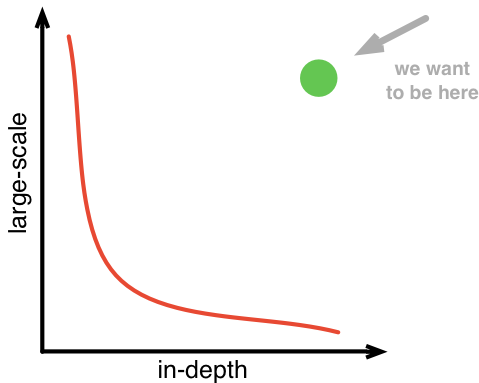
\includegraphics[width=3.5in]{figures/related/sota_analysis.png}
\caption{A visualisation of the current state of the art of preservation analysis tools in relation to the volume of content and the depth of the analysis.}
\label{fig:sota_analysis}
\end{center}
\end{figure}

\section{Tool Support}
%talk about meta data tool support
%preservation planning tool support and automation and scalability
%content profiling/ format profiling tool support
%repositories, monitoring services
Due to the rising awareness of digital preservation and the numerous projects conducted in this area in recent years, many existing tools have found new use and many new tools were written from scratch in order to support DP activities. This section provides a short overview of some of the more prominent ones that are related to content profiling.

A recent report (created as part of the SCAPE project) summarises an evaluation framework and the results of the tests of several identification and characterisation tools \cite{Knijff:2011it}. It provides a rather good overview of the current state of the art of such tools but concentrates mostly on their identification capabilities. In the report six tools (DROID 6.0\footnote{http://sourceforge.net/projects/droid/}, FIDO\footnote{https://github.com/openplanets/fido}, Unix File Tool\footnote{http://unixhelp.ed.ac.uk/CGI/man-cgi?file}, FITS\footnote{http://code.google.com/p/fits/} 0.5 and JHOVE2\footnote{https://bitbucket.org/jhove2/main/wiki/Home}) were evaluated against 22 criteria among which, the tool interface, its license type, platform dependencies, accuracy of reported results, documentation, etc. Another recent research conducted by the National Library of Australia has investigated four file identification tools (File Investigator Engine\footnote{http://www.forensicinnovations.com/fiengine.html}, Outside-In File ID\footnote{http://docs.oracle.com/cd/E16184\_01/dev.837/e12875/title.htm}, FIDO and file) and five metadata extraction tools (File Investigator Engine, Exiftool\footnote{http://owl.phy.queensu.ca/~phil/exiftool/}, MediaInfo\footnote{http://mediainfo.sourceforge.net/en}, pdfinfo\footnote{http://www.foolabs.com/xpdf/download.html} and Apache Tika\footnote{http://tika.apache.org}), some of which commercial. The results of these tests can be found in \cite{NLASP2452}.

Here we summarise the strengths and weaknesses of some of these and other tools briefly in order to give an overview of the current state of the art.

\begin{itemize}
\item \textbf{DROID 6.0}\newline
Droid is an identification tool produced by the National Archives, which uses the PRONOM\footnote{http://nationalarchives.gov.uk/pronom/} registry and its format signatures and/or file extensions. It provides information about the mime type, format and format version of a file as long it is in the DROID signature file, which contains the 'magic numbers' of the PRONOM registry. It also outputs a PRONOM Unique Identifier or PUID, which can be used to trace the format back into the registry.
Unfortunately, the registry is not open and its maintenance is slow. However, the tool is very useful and widely adopted within the DP community.

\item \textbf{Apache TIKA}\newline
Tika is an open source project from The Apache Software Foundation that is able to extract metadata from files with various formats. It is a stable tool able to identify files by analysing their bitstream and allows the deeper characterisation of some of these files.  

\item \textbf{FIDO}\newline
FIDO is another identification tool that is a clone of Droid and also uses the PRONOM signature file registry. Although it has numerous glitches, FIDOs performance proves to be 35 times faster than DROID when working on one file at a time.

\item \textbf{UNIX File Tool}\newline
File is a CLI utility application included in every Unix distribution and first released in 1973. The tool has stood the test of time and has proven to be very stable, which also makes it widely adopted in the DP community. It makes use of magic numbers to identify files and has been used in DP activities for a long time. It has a very good computational performance and supports large number of formats.

\item \textbf{FITS} \newline
The File Information Tool Set is developed by the Harvard University Library. It wraps common identification and characterisation tools as the ones described here and tries to consolidate them and provide a normalised output. By providing basic provenance information for each extracted record it combines the consolidation result and provides a very basic confidence status for the extracted value of each property. This proves to be helpful for cases where there are uncertainties. The framework is designed to be extended, so that other tools can be also added. The tool seems very helpful, although there are some instabilities and problematic cases.

\item \textbf{JHOVE}\newline
JHOVE is one of the most well-known identification and characterisation tools used by the DP community. It is also developed by the Harvard University Library and is able to extract meta data from various formats based on different modules. Probably one of the most valuable features of JHOVE is the ability the check a file for wellformedness and validity against the format specification.

\item \textbf{JHOVE 2}\newline
JHOVE 2 is a successor project for the JHOVE tool and also provides an extensible architecture for characterisation tools and modules. It is developed as an open source tool by the California Digital Library, Portico and Stanford University. Currently it produces helpful output only for a few types of documents as the different modules are not yet developed.

\end{itemize}

Although this list is not complete, and there are many other tools that are able to extract meta data as well, it shows that the current state of the art is able to provide enough meta data that could be used as input for various preservation activities. The tools have their downsides in terms of format coverage and/or performance, but still provide very valuable information.
Currently there are only a few tools however, that are able to analyse collections. PRONOM ROAR, for example, is able to create a format profile within a repository interface with the help of DROID.
Various repositories provide basic information as the formats and size of objects, however no further stratification is possible, although the characterisation data is present.
PLATO provides excellent decision making support by utilising different means, but still handles the content profiling step as a high-level non-automated task, which increases the risk of bias during experimentation and analysis.
Nonetheless, the means for in-depth analysis on larger-scale are present and seem to be feasible, although there are various issues that still have to be overcome.
% what is present.
% explain that the tools for different types of contents are there, but no tool does
% collection profiling
% scape evaluation of characterisation...

\section{Quality Assurance of Measures}
One of the biggest downsides of all identification and characterisation tools is the lack of quality assurance processes. Often there is no way to verify if an extracted measurement value is really representing the truth. This is a huge problem, as it is hard to make assumptions about correctness without having a ground truth in the first place.
Some tools such as FITS try to tackle this problem on a very basic level by stating a confidence level in the form of an enumeration (OK, SINGLE\_RESULT, PARTIAL, CONFLICT). It is not perfect, but it provides the user with warnings about potential threats.
A big problem here is the consolidation. Often tools provide the same measurement for a specific property but the output format is slightly different. This makes it hard for an automatic consolidator to decide if the values are equal or not. Thus the problem of quality assurance depends on external information provided by other processes or even by manual verification. 
Clearly, this is a hard, tedious and long running process and thus it is (partially) neglected.
Nonetheless, it is an essential precondition in order to assure correct input data for the analysis.
% despite the tools there is a big gap
% tools extract some measures, but there is almost no way, to assure that
% a measurement is correct
% often tools extract the same information and represent it in different way, thus providing a conflict - verification is hard...
% JHove validation, verification


\section{Observations}
In order to prepare a preservation action plan some prerequisites have to be met. The following provides a simplified list of steps that would occur in a common digital preservation scenario, usually in the following order: 
\begin{enumerate}
\item Organisational policies about the management of the content are created and curated.
\item A monitoring component is used to observe the policies and operations over the content for violations.
\item As part of the repository ingest, an identification and deep characterisation process extracts valuable meta data and stores it within the repository.
\item A content profile is generated and exported for other tools.
\item A monitoring component identifies that a certain subset of objects violates the policies and notifies a planning expert for the potential threat.
\item A planner uses the content profile, a profiler to analyse and stratify the content into smaller homogeneous partitions as well as identify representative sample objects for the partitions.
\item A planning tool is used to validate the threat and to create an action plan that is able to cope with the policy violations.
\item The action plan is submitted to a repository, which knows how to execute the described preservation action.
\item The monitoring component observes the operations of the repository and notifies the interested parties of important events, such as throughput, failures and task executions. 
\item The violation is taken care of and the monitor component continues its work.
\end{enumerate}

The state of the art provides some of these components and actors in this high-level workflow. Any organisation actively doing digital preservation has its own set of policies of how to handle different types of content. The problem here is that often such policies are just high-level descriptive statements, which are not structured in any specific form and thus are not machine readable. This makes it almost impossible to use in automated fashion. Also there are numerous repositories that can manage digital objects and extract meta data from them. 

The planning tool PLATO provides the needed facilities to create an action plan.

However, a couple of components are missing. A preservation monitor, that scans relevant properties of the world and evaluates their values for changes, eventually notifying users or other agents of interesting events. Such a monitor is currently developed within the SCAPE Project \cite{becker-ipres2012}.
Another crucial part that is missing is an method able to profile a massive content set and stratify it into smaller homogeneous and manageable partitions. Such a framework would provide two main benefits. First, analysis and content stratification and thus better foundation for planning experiments with reduced bias. And second input to a preservation monitor that will be able to create a global profile of content, which would be of great benefit to the DP community.

% summarize, what is going on,
% what is missing
% what is the problem of the current state of the art
% based on the research you made.